\section{Optimizing the LS$^{2}$ simulation engine}
\label{Implementation}
In the following section I will describe how I optimized the LS$^{2}$ simulation engine using mainly SSE intrinsics. I will begin introducing the software itself and its research purpose. Then, I will document the approach taken for development, including information about how I benchmarked the application in order to acquire meaningful results. The main part of this section will be comprised of a detailed explanation of the optimized source code of the three algorithms that I have chosen to improve.
\subsection{LS$^{2}$: A simulation engine for lateration algorithms}

The term "lateration algorithms" is commonly used to refer to geometric algorithms that use distance measurements to determine the location of points in the plane or in a three-dimensional space (as opposed to triangulation which uses the measurement of angles). The most basic representative of this group of algorithms is known as \emph{trilateration}: Obviously, in the euclidean plane it needs at least three known spots (subsequently called \emph{anchors}) and the distance measurements hereof to be able to narrow down the current position to a single point. Relative to each of the anchors, this point lies on a circle that has its center on the anchor and the distance as its radius. Trilateration determines the current position by solving these three linear equations, in other words, it calculates the intersection of the three circles drawn around the anchors. In real-world applications such as the Global Positioning System (GPS), distance measurements, like all physically measured data, are generally error-prone. Most commonly, distances are estimated by measuring the time it takes a signal (e.g. light, radio) to travel between an anchor and the client. Because of these erroneous distances, circles drawn around the anchors do not necessarily intersect at a single point and the basic trilateration algorithm fails to produce an exact result. In order to calculate an approximation of the current position, trilateration can be adapted to return the geometric center of the now up to three circle intersections. However, during the last decades, several superior, more complex algorithms have been created in order to provide improved position estimations based on error-prone distances.

The \emph{FU Berlin Parallel Lateration-Algorithm Simulation and Visualization Engine} (LS$^{2}$), written by Heiko Will, Thomas Hillebrandt, and Marcel Kyas and first presented at the WPNC conference 2012, is a graphical evaluation framework for lateration algorithms. As the authors explain in~\cite{will2012ls2}, the application's fundamental idea is to not only calculate an average algorithm error based on randomized locations, which has been the main evaluation criterium for lateration algorithms so far, but to calculate errors for all locations on a given "playing field" in parallel and in the end to provide the user with an image displaying the so-called \emph{spatial position error distribution}. The assumption is that the position of the anchors has significant influence on the algorithm's performance, even more so than the errors of the distances. 

The application is divided into three main parts: The engine itself, responsible for distributing the work load and calculating the position errors, a set of error models, which are used to simulate the distance measurement errors, and the lateration algorithms. Parametrized with a set of anchor positions, the error model, and the desired algorithm, the engine first starts a number of threads and associates them with a spatial slice of the 1000x1000 playing field. For each position in its slice, a thread calculates the real distance between the position and the anchors, randomly modifies the distances according to the error model, and executes the lateration algorithm. It then calculates the algorithm error as the difference between the real distance and the algorithm's return value. This process is repeated 40 times for each position, before the resulting average error is written back to an image buffer.


\begin{itemize}
\item explain liblat; goals, functionality
\item cite heiko
\item bla~\cite{will2012ls2}
\end{itemize}
\subsection{Approach}
\subsubsection{Benchmarking}
blablabla \ref{fig:branchtree}

\begin{figure}[h]
\begin{center}
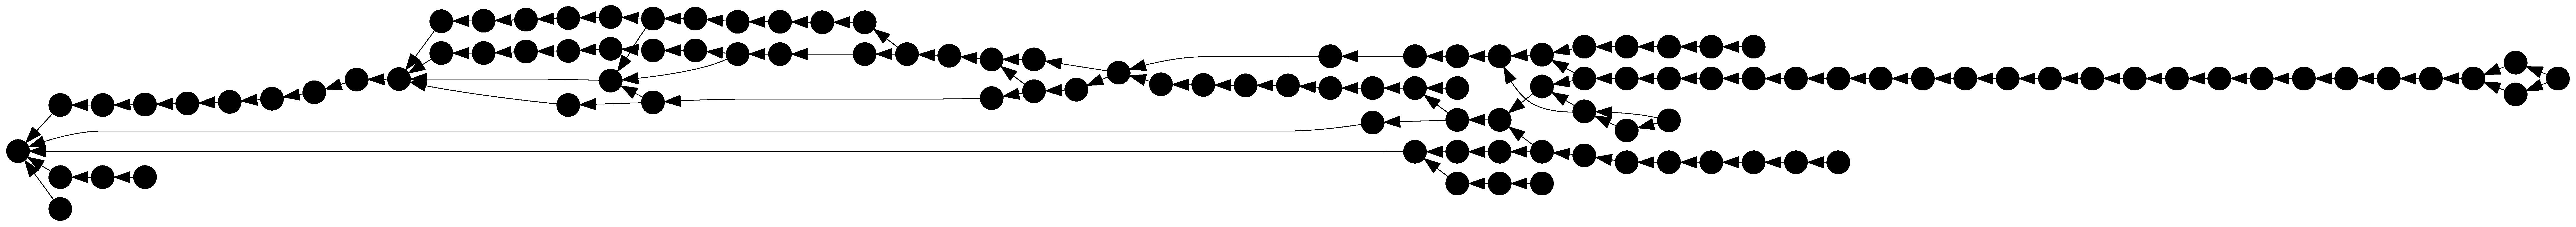
\includegraphics[width=14cm]{img/branchtree}
\end{center}
\caption{Visualization of \texttt{git} history}
\label{fig:branchtree}
\end{figure}

\begin{itemize}
\item simple benchmarking using \texttt{time}
\item profiling using valgrind, cachegrind.
\item maybe explain benchlat
\item difficulties related to benchmarking:
\begin{itemize}
\item different input leads to \emph{extremly} fluctuating results; don't optimize for a single case!
\item random input coordinates; uniform distribution
\end{itemize}
\end{itemize}
\subsubsection{Other tools and hardware (?)}
\begin{itemize}
\item read assembly once in a while 
\item version control software for backtracking
\item used software versions and hardware



\end{itemize}
\subsection{Algorithm 1: geolat}
\subsection{Algorithm 2: aml}
\subsection{Framework}
--> movntps yyx